\documentclass[herrin-thesis.tex]{subfiles}
\begin{document}

\chapter{Light Collection Efficiency}
\label{app:lightmap}

\section{Motivation}
Two events with the same energy occurring in different locations in the liquid xenon will not necessarily produce the same signal. This will lead to a degraded energy resolution. For example, an event occurring near a corner of the detector will have more light escape through the gap between the PTFE reflectors and the APD platter. Additionally, while the trim voltages applied to each APD gang attempt to normalize the performance, there is still a 2.5\% spread in the response. While the latter can potentially be accounted for with measurements using the laser pulser system, the system was operating for Run 2a. Such a correction, however, would still not correct for geometric efficiency.

Although attempts have been made to simulate light collection in the detector (see, for example \cite{Mackay:2011fk}), this takes a very thorough understanding of the detector construction and the response of all materials to \SI{178}{\nm} light. Individually tracking photons is also extremely computationally intensive. Therefore, data from source calibrations is used to map out the light response of the detector.

\section{Building the light map}
\subsection{Calibration Runs}
In order to illuminate the entire detector, long calibration runs at both anode positions and all three cathode locations are needed. These

\subsection{Event Selection}
Only single site full-absorption events are used to make the light map, since both their location and energies are known. Full absorption events are identified by looking at the ionization spectrum. The mean and sigma of the full-absorption peak are fit with a Gaussian + complementary errror function model like that used for calibration. Only events with ionization energies between \(+0.33\sigma\) and \(+3.0\sigma\) are used. This cut retains 37\% of the full-absorption events, and should only retain 3\% of the Compton scatter events with energies within 2\(\sigma\) of the peak. Since scintillation is correlated with ionization, and the ionization response is uniform throughout the detector (after electron lifetime and shielding grid corrections), this should give a give a sample of events with the same scintillation throughout the detector.

\subsection{Binning the Detector Volume}

The detector volume is divided into 1352 spatial bins. This binning is split into 8 \(\phi\) bins, 13 radial bins, and 13 \(z\) bins. The \(\phi\) binning is evenly-spaced. For the \(z\) binning, the TPC is divided evenly into 11 slices. The central slice is then divided into 3 even slices, since the response is observed to change rapidly near the cathode. The radial binning consists of 1 bin from \SIrange{0}{3}{\mm}, bins every \SI{20}{mm} from \SIrange{30}{90}{\mm}, bins every \SI{10}{\mm} from \SIrange{90}{120}{\mm}, and bins every \SI{8}{mm} from \SIrange{120}{168}{\mm}. This binning is chosen to ensure adequate statistics within all bins, and to optimally map the response in regions with a high light collection gradient.

Full absorption, single site events from all calibrations are placed into the bins according to the event location. Then the mean of each bin is stored in a 3-dimensional histograms. This histogram stores the scintillation response in each bin of the detector and is referred to as the ``light map''. It is stored in a database. \Cref{fig:lightmap_binned_phi_slices,fig:lightmap_binned_z_slices} show an example light map. Histograms of the number of events in each bin, and the error on the mean, are also retained to ensure an adequate amount of data was used.

\section{Correction Function}

\subsection{Trilinear interpolation in cylindrical polar coordinates}
Suppose a function \(F(r_i, \phi_j, z_k)\) is defined only at discrete points, and \(f(r, \phi, z)\) is a smooth transition between the defined points of \(F\). The simplest way to do so is with trilinear interpolation. Define
\begin{equation}
r_d = \frac{r_{i+1} - r_{i}}{r_{i+1}+r_{i}} ; \phi_d = \frac{\phi_{j+1} - \phi_{j}}{\phi_{j+1}+\phi_{j}}; z_d = \frac{z_{k+1} - z_{k}}{z_{k+1}+z_{k}}
\label{eq:lightmap_interpolation_weights}
\end{equation}
where \(r_i \leq r < r_{i+1}\) and \(z_k \leq z < z_{k+1}\). In cylindrical coordinates, \(\phi\) is cyclical, and so \(\phi\) lies between \(\phi_j\) and \(\phi_{j+1} \mod 2\pi\). Multiples of \(2\pi\) may need to be added or subtracted from the angles at which \(F\) is defined to ensure \(0 \leq \phi_d < 1\).

Now \(f\) can be constructed:
\begin{align}
f(r, \phi, z) &=&   & F(r_{i\phantom{+1}}, \phi_{j\phantom{+1}}, z_{k\phantom{+1}}) (1-r_d)(1-\phi_d)(1-z_d)	\nonumber\\
		& & + & F(r_{i\phantom{+1}}, \phi_{j\phantom{+1}}, z_{k+1})		     (1-r_d)(1-\phi_d)z_d 		\nonumber\\
		& & + & F(r_{i\phantom{+1}}, \phi_{j+1},		      z_{k\phantom{+1}}) (1-r_d)\phi_d(1-z_d)		\nonumber\\
		& & + & F(r_{i\phantom{+1}}, \phi_{j+1}, 		      z_{k+1})		     (1-r_d)\phi_d z_d			\nonumber\\
		& & + & F(r_{i+1}, 		     \phi_{j\phantom{+1}}, z_{k\phantom{+1}}) r_d(1-\phi_d)(1-z_d)		\nonumber\\
		& & + & F(r_{i+1}, 		     \phi_{j\phantom{+1}}, z_{k+1})		     r_d(1-\phi_d)z_d			\nonumber\\
		& & + & F(r_{i+1}, 		     \phi_{j+1}, 		      z_{k\phantom{+1}})  r_d\phi_d(1-z_d)			\nonumber\\
		& & + & F(r_{i+1},		     \phi_{j+1}, 		      z_{k+1})		      r_d\phi_dz_d
\label{eq:lightmap_trilinear}
\end{align}

There is a complication, however, when the lower neighbor bin for \(r\) is the \(z\)-axis. In order to ensure that \(f\) is single-valued at \(r=0\), define the value of \(F\) at the axis as the mean value for the surrounding points: 
\begin{equation}
F(r_{0}=0, \phi, z_k) = \frac{1}{N_\phi}\sum_{j=1}^{N_\phi} F(r_{1}, \phi_j, z_k)
\end{equation}

Then \cref{eq:lightmap_trilinear} can still be used. In this case, \(\phi_d\) will not matter in the terms involving \(r_i\).

\subsection{Correcting for Light Response}

To correct for the light response, first the histogram containing the light map is normalized such that the average response is 1. Let \(F(r_i, \phi_j, z_k)\) be the value of the normalized light map for the bin that has center \((r_i, \phi_j, z_k)\). Then let \(f(r,\phi,z)\) be the trilinear interpolation of \(F\). \Cref{fig:lightmap_correction_phi_slices,fig:lightmap_correction_z_slices} show an example of this interpolation. The normalized scintillation response for an event is
\begin{equation}
g = \frac{\sum_{m=1}^{N}E_m f(r_m, \phi_m, z_m)}{\sum_{m=1}^{N}E_m}
\label{eq:lightmap_weighted_response}
\end{equation}
where the sums are over the \(N\) ionization clusters in the event, each with a position \((r_m, \phi_m, z_m)\) and an ionization energy \(E_m\). This assumes that the fraction of total scintillation light produced by a charge cluster at a given position is the same as that cluster's fraction of total ionization energy.

If \(E_{s}\) is the uncorrected scintillation signal, then
\begin{equation}
E_{s,\text{corrected}} = \frac{E_s}{g}
\label{eq:lightmap_corrected_signal}
\end{equation}
is the corrected signal.

\begin{sidewaysfigure}[p]
\centering
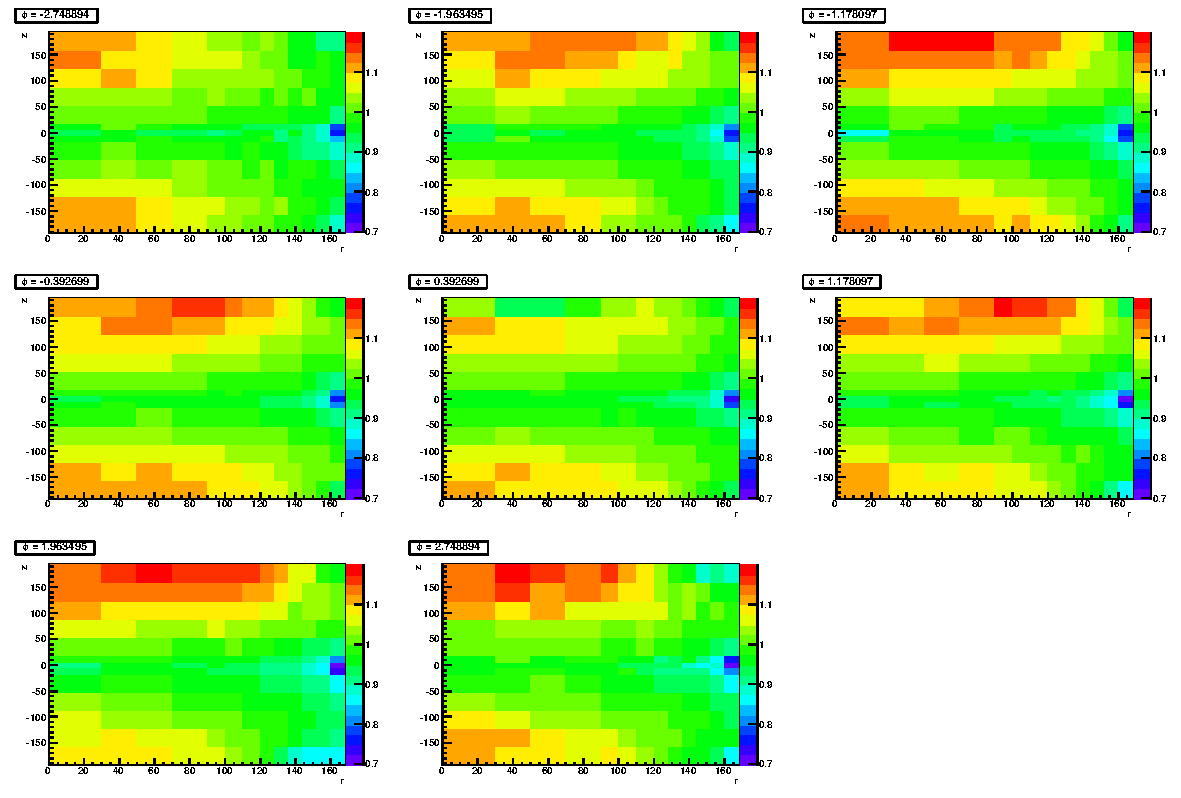
\includegraphics[width=\textwidth]{./plots/lightmap_binned_phi_slices.pdf}
\caption[Lightmap \(\phi\) slices]{The lightmap, showing the bins in \(r\) (horizontal axis) and \(z\) (vertical axis) for each of the 8 \(\phi\) bins. Note the finer binning around the cathode at \(z=0\).}
\label{fig:lightmap_binned_phi_slices}
\end{sidewaysfigure}

\begin{sidewaysfigure}[p]
\centering
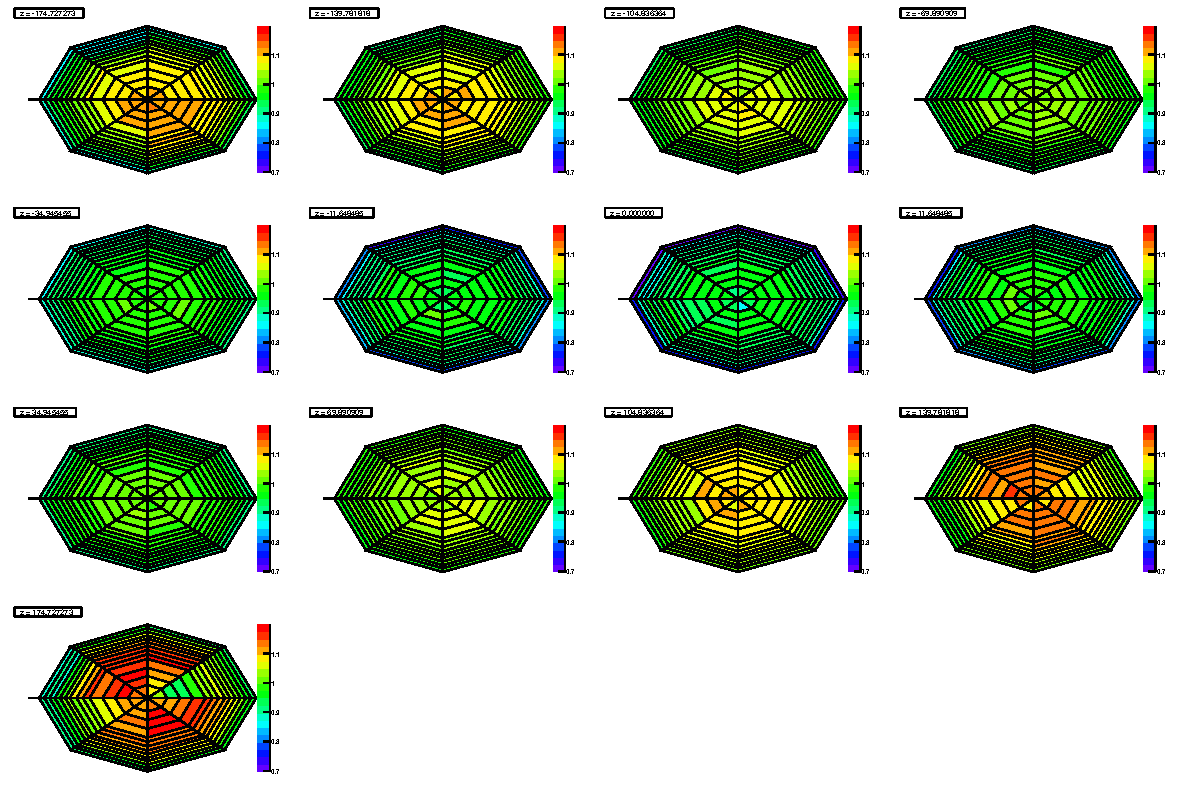
\includegraphics[width=\textwidth]{./plots/lightmap_binned_z_slices.pdf}
\caption[Lightmap \(z\) slices]{The lightmap, showing the bins in \(r\) and \(\phi\) for each of the 13 \(z\) bins.}
\label{fig:lightmap_binned_z_slices}
\end{sidewaysfigure}

\begin{sidewaysfigure}[p]
\centering
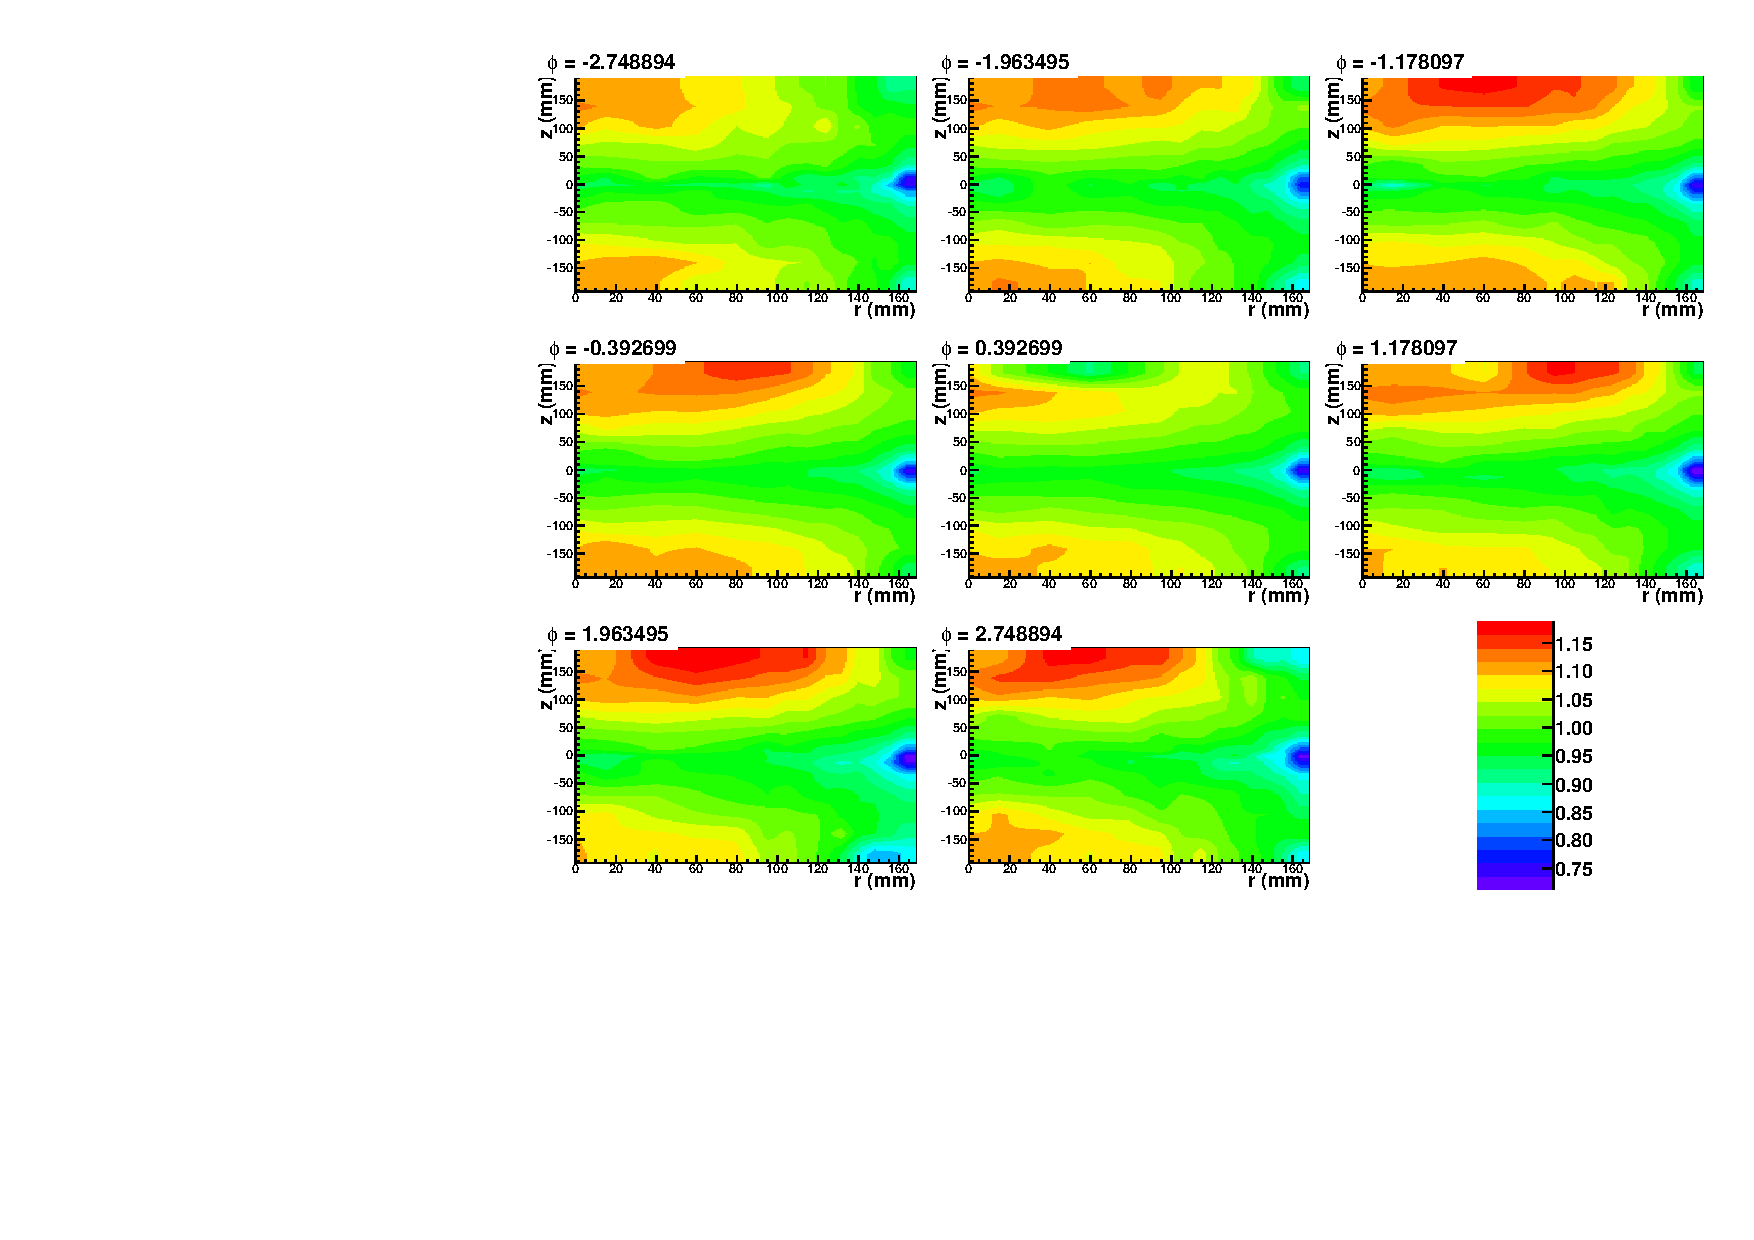
\includegraphics[width=\textwidth]{./plots/lightmap_correction_phi_slices.pdf}
\caption[Correction function \(\phi\) slices]{The light response function \(f(r,\phi,z)\), evaluated at 8 discrete values of \(\phi\) over the full range of \(r\) (horizontal axis) and \(z\) (vertical axis).}
\label{fig:lightmap_correction_phi_slices}
\end{sidewaysfigure}

\begin{sidewaysfigure}[p]
\centering
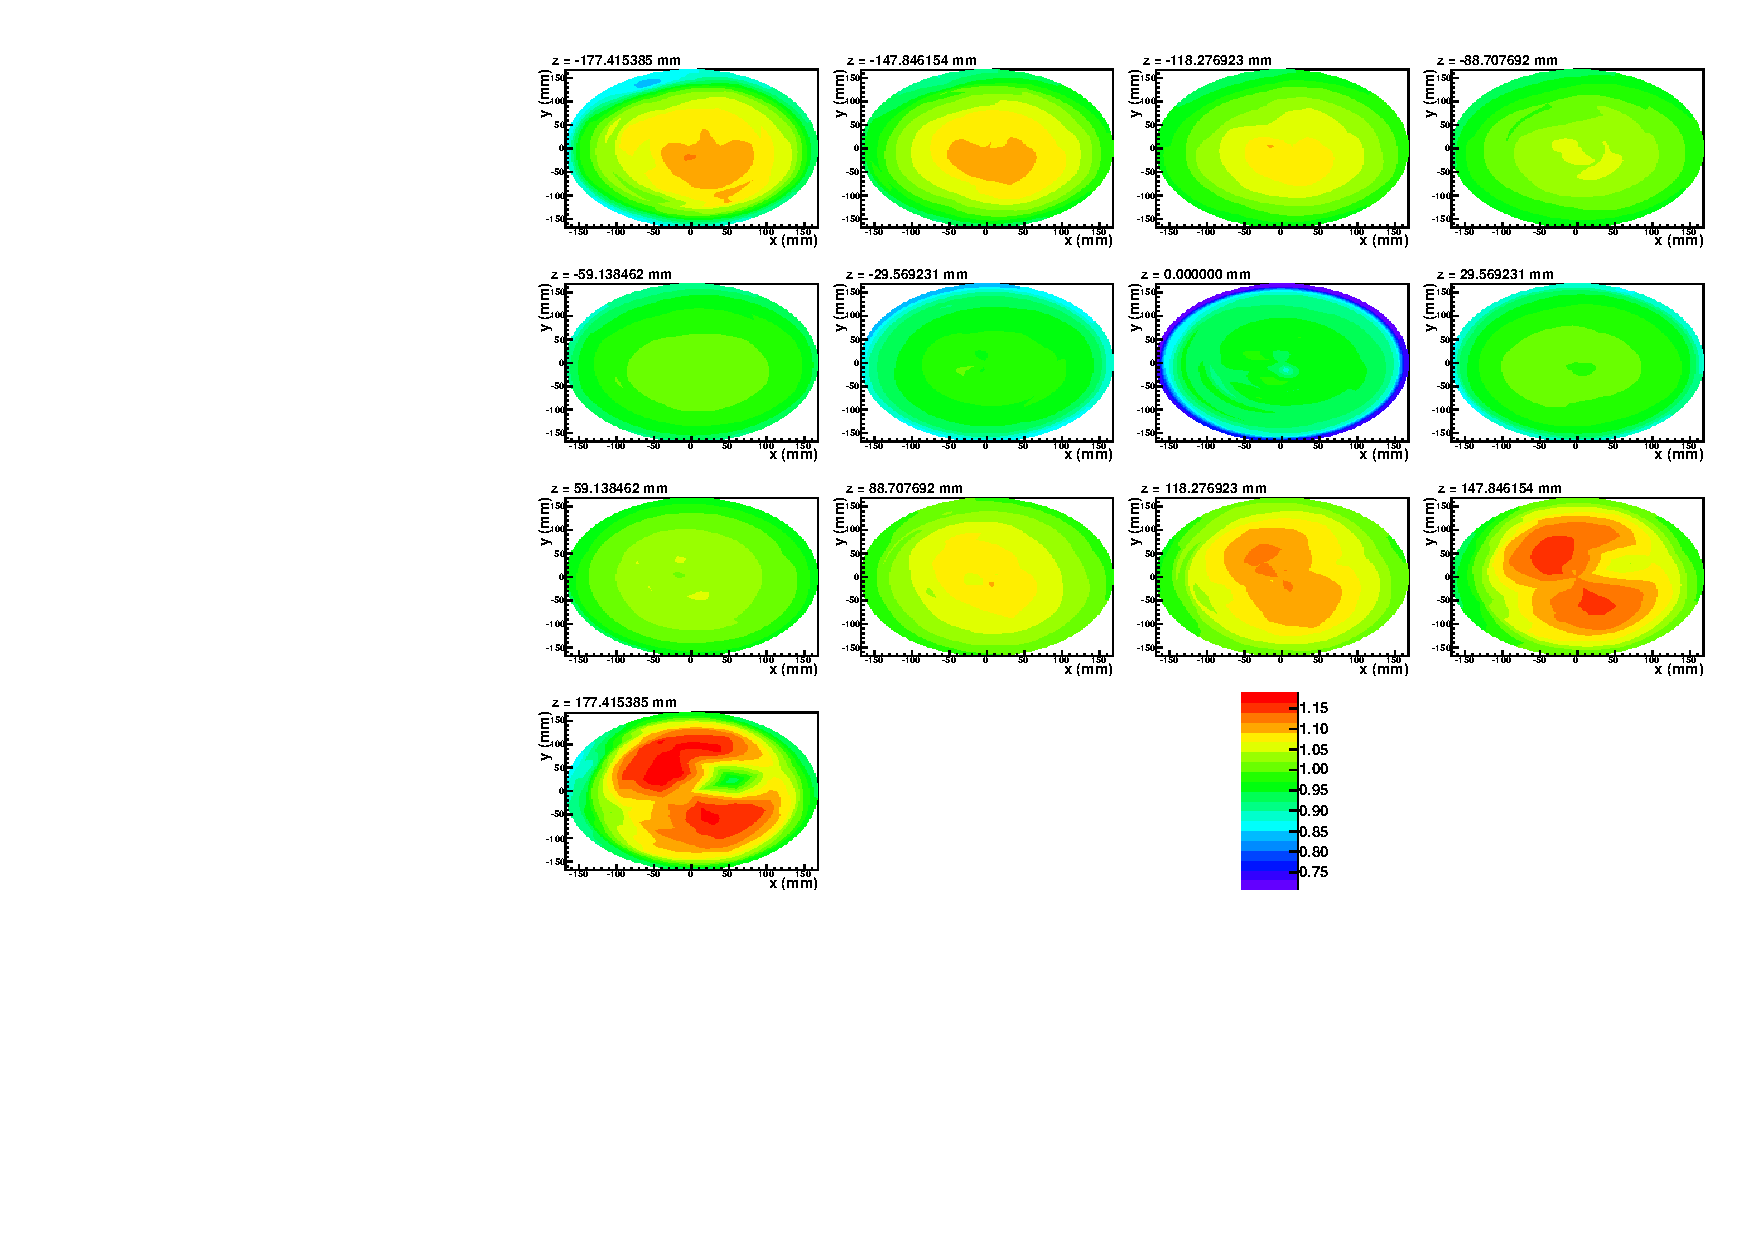
\includegraphics[width=\textwidth]{./plots/lightmap_correction_z_slices.pdf}
\caption[Correction function \(z\) slices]{The light response function \(f(r,\phi,z)\), evaluated at 13 discrete values of \(z\) over the full range of \(x\) (horizontal axis) and \(y\) (vertical axis). Notice that the most light is collected for events near the anodes. Near the \(+z\) anode, just above the \(+x\) axis there is a region of low collection due to a disabled APD gang.}\label{fig:lightmap_correction_z_slices}
\end{sidewaysfigure}

\end{document}
